\begin{center}
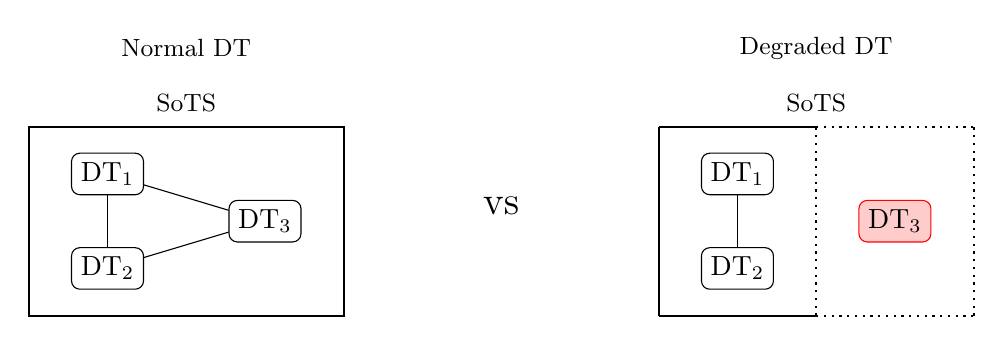
\begin{tikzpicture}[
dt/.style={draw, rounded corners=3pt, fill=white, minimum width=0.9cm}
]

% ---------- LEFT: NORMAL ----------
\node at (0,3) {\small Normal DT};

% SoTS boundary
\fill[white] (-2,-0.4) rectangle (2,2);
\draw[thick] (-2,-0.4) rectangle (2,2);
\node at (0,2.3) {\small SoTS};

% DTs
\node[dt] (dt1) at (-1,1.4) {DT$_1$};
\node[dt] (dt2) at (-1,0.2) {DT$_2$};
\node[dt] (dt3) at (1,0.8) {DT$_3$};

% connections
\draw (dt1) -- (dt2);
\draw (dt1) -- (dt3);
\draw (dt2) -- (dt3);

% ---------- VS ----------
\node at (4,1) {\Large vs};

% ---------- RIGHT: DEGRADED ----------
\node at (8,3) {\small Degraded DT};

% SoTS outer boundary
\draw[thick] (6,-0.4) -- (8,-0.4);
\draw[thick] (6,-0.4) -- (6,2);
\draw[thick] (6,2) -- (8,2);

% partition
\draw[dotted, thick] (8,-0.4) -- (8,2);

% degraded boundary
\draw[dotted, thick] (8,-0.4) -- (10,-0.4);
\draw[dotted, thick] (10,-0.4) -- (10,2);
\draw[dotted, thick] (8,2) -- (10,2);

\node at (8,2.3) {\small SoTS};

% functional active region
\fill[white] (6.1,-0.3) rectangle (7.9,1.9);

% active DTs
\node[dt] (dt1b) at (7,1.4) {DT$_1$};
\node[dt] (dt2b) at (7,0.2) {DT$_2$};

\draw (dt1b) -- (dt2b);

% degraded DT
\node[dt, draw=red, fill=red!20] (dt3b) at (9,0.8) {DT$_3$};

\end{tikzpicture}
\end{center}

\begin{center}
{\footnotesize
\tikz{\draw[red, thick, fill=red!20] (0,0) rectangle (0.25,0.25);} faulty DT}
\end{center}